\chapter{Kravspecifikation}
Ud fra systembeskrivelsen er der formuleret en række krav til projektet. Disse indebærer to use cases og et antal ikke-funktionelle krav. Følgende afsnit beskriver aktøren for systemet samt de krav der er sat til systemet.

\section{Aktørbeskrivelse}
På figur \ref{fig:useCaseDiagram} ses use case diagrammet for systemet. På figuren ses det at der er én primær bruger for systemet; brugeren. 

\begin{figure}[H]
	\centering
	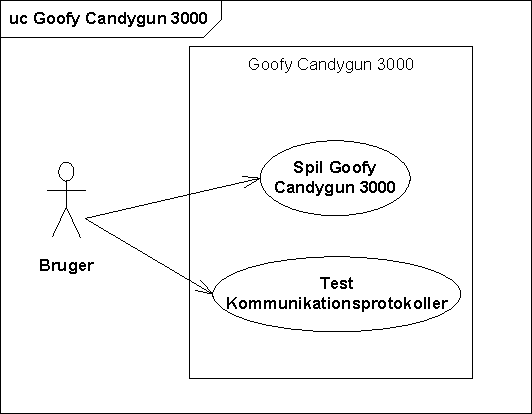
\includegraphics[width=0.80\textwidth]{Kravsspecifikation/images/usecaseDiagram}
	\caption{Use case diagram}
	\label{fig:useCaseDiagram}
\end{figure}

\noindent På tabel \ref{table:actor} vises aktørbeskrivelsen for brugeren for systemets use cases. 
\begin{table}[H]
	\begin{tabularx}{\textwidth}{| p{2cm} | p{9.1cm} |}
		\hline
		Aktørens Navn: & Bruger \\ 
		\hline
		Alternativ Navn: & Spiller \\
		\hline
		Type: & Primær \\
		\hline
		Beskrivelse: & Brugeren initierer Goofy Candygun 3000 samt starter systemtesten. Derudover har brugeren mulighed for at stoppe spillet igennem brugergrænsefladen. Brugeren vil under spillet interagere med Goofy Candy Gun gennem Wii-Nunchucken.
		\\ \hline
	\end{tabularx}
	\caption{Aktørbeskrivelse for brugeren}
	\label{table:actor}
\end{table}


\newpage
\section{Use case beskrivelse}
I dette afsnit er der en kort beskrivelse af systemets use cases og dets ikke-funktionelle krav. De fully dressed use cases kan findes i dokumentationen, afsnit 1.4- \textit{Fully Dressed Use Cases} side \#ref.

\subsection{Use case 1}
Brugeren initierer use casen ved at starte spillet via brugergrænsefladen og vælge spiltype; oneplayer eller partymode. Herefter vælges antallet af skud i et spil og disse puttes i magasinet. Når dette er gjort kan spillet påbegyndes. Brugeren indstiller kanonen med Wii-nunchuck og affyrer den. Herefter lader systemet et nyt skud og samme procedure gentages. Til slut vises information om spillet på brugergrænsefladen. Brugeren afslutter spillet ved at trykke på Exit-knappen på brugergrænsefladen og denne vender tilbage til starttilstanden. 

\subsection{Use case 2}
Brugeren initierer use casen ved starte systemtesten via brugergrænsefladen. Herefter testes forbindelserne mellem hardwareblokkene forbundet via systemets busser. Hvis der sker fejl under systemtesten, raporteres disse til brugeren via brugergrænsefladen og use casen afbrydes. Ved en successfuld systemtest, rapporteres dette til brugeren via brugergrænsefladen.

\section{Ikke-funktionelle krav}
Til beskrivelse af produktets specifikationer er der udarbejdet nogle ikke-funktionelle krav. Kravene omhandler produktets dimensioner, kanonens rotationsevner og kanonens affyring. De ikke funktionelle krav findes i dokumentationen afsnit 1.5 - \textit{Ikke funktionelle krav} side \#ref.

\section{Accepttestspecifikation}
Ud fra systemets use cases og ikke-funktionelle krav, er der blevet udarbejdet en accepttestspecifikation, for at verificere systemets funktionaliteter, efter endt udviklingsforløb. Denne kan findes i dokumentationen afsnit 2 - \textit{Accepttestspecifikation} side \#ref. 